%! TEX program = xelatex
%! TEX root = ../root.tex

\section{实验步骤与调试}
\subsection{仿真} 根据已经写好的代码,进行仿真模拟\\
\subsubsection{异常处理}
当程序遇到exception时,跳入处理程序。程序在WB阶段接收exception信号,并跳入异常处理程序,将还在执行的命令全部清空,并取消寄存器的写入。
\begin{figure}[H] %H为当前位置,!htb为忽略美学标准,htbp为浮动图形
	\centering %图片居中
	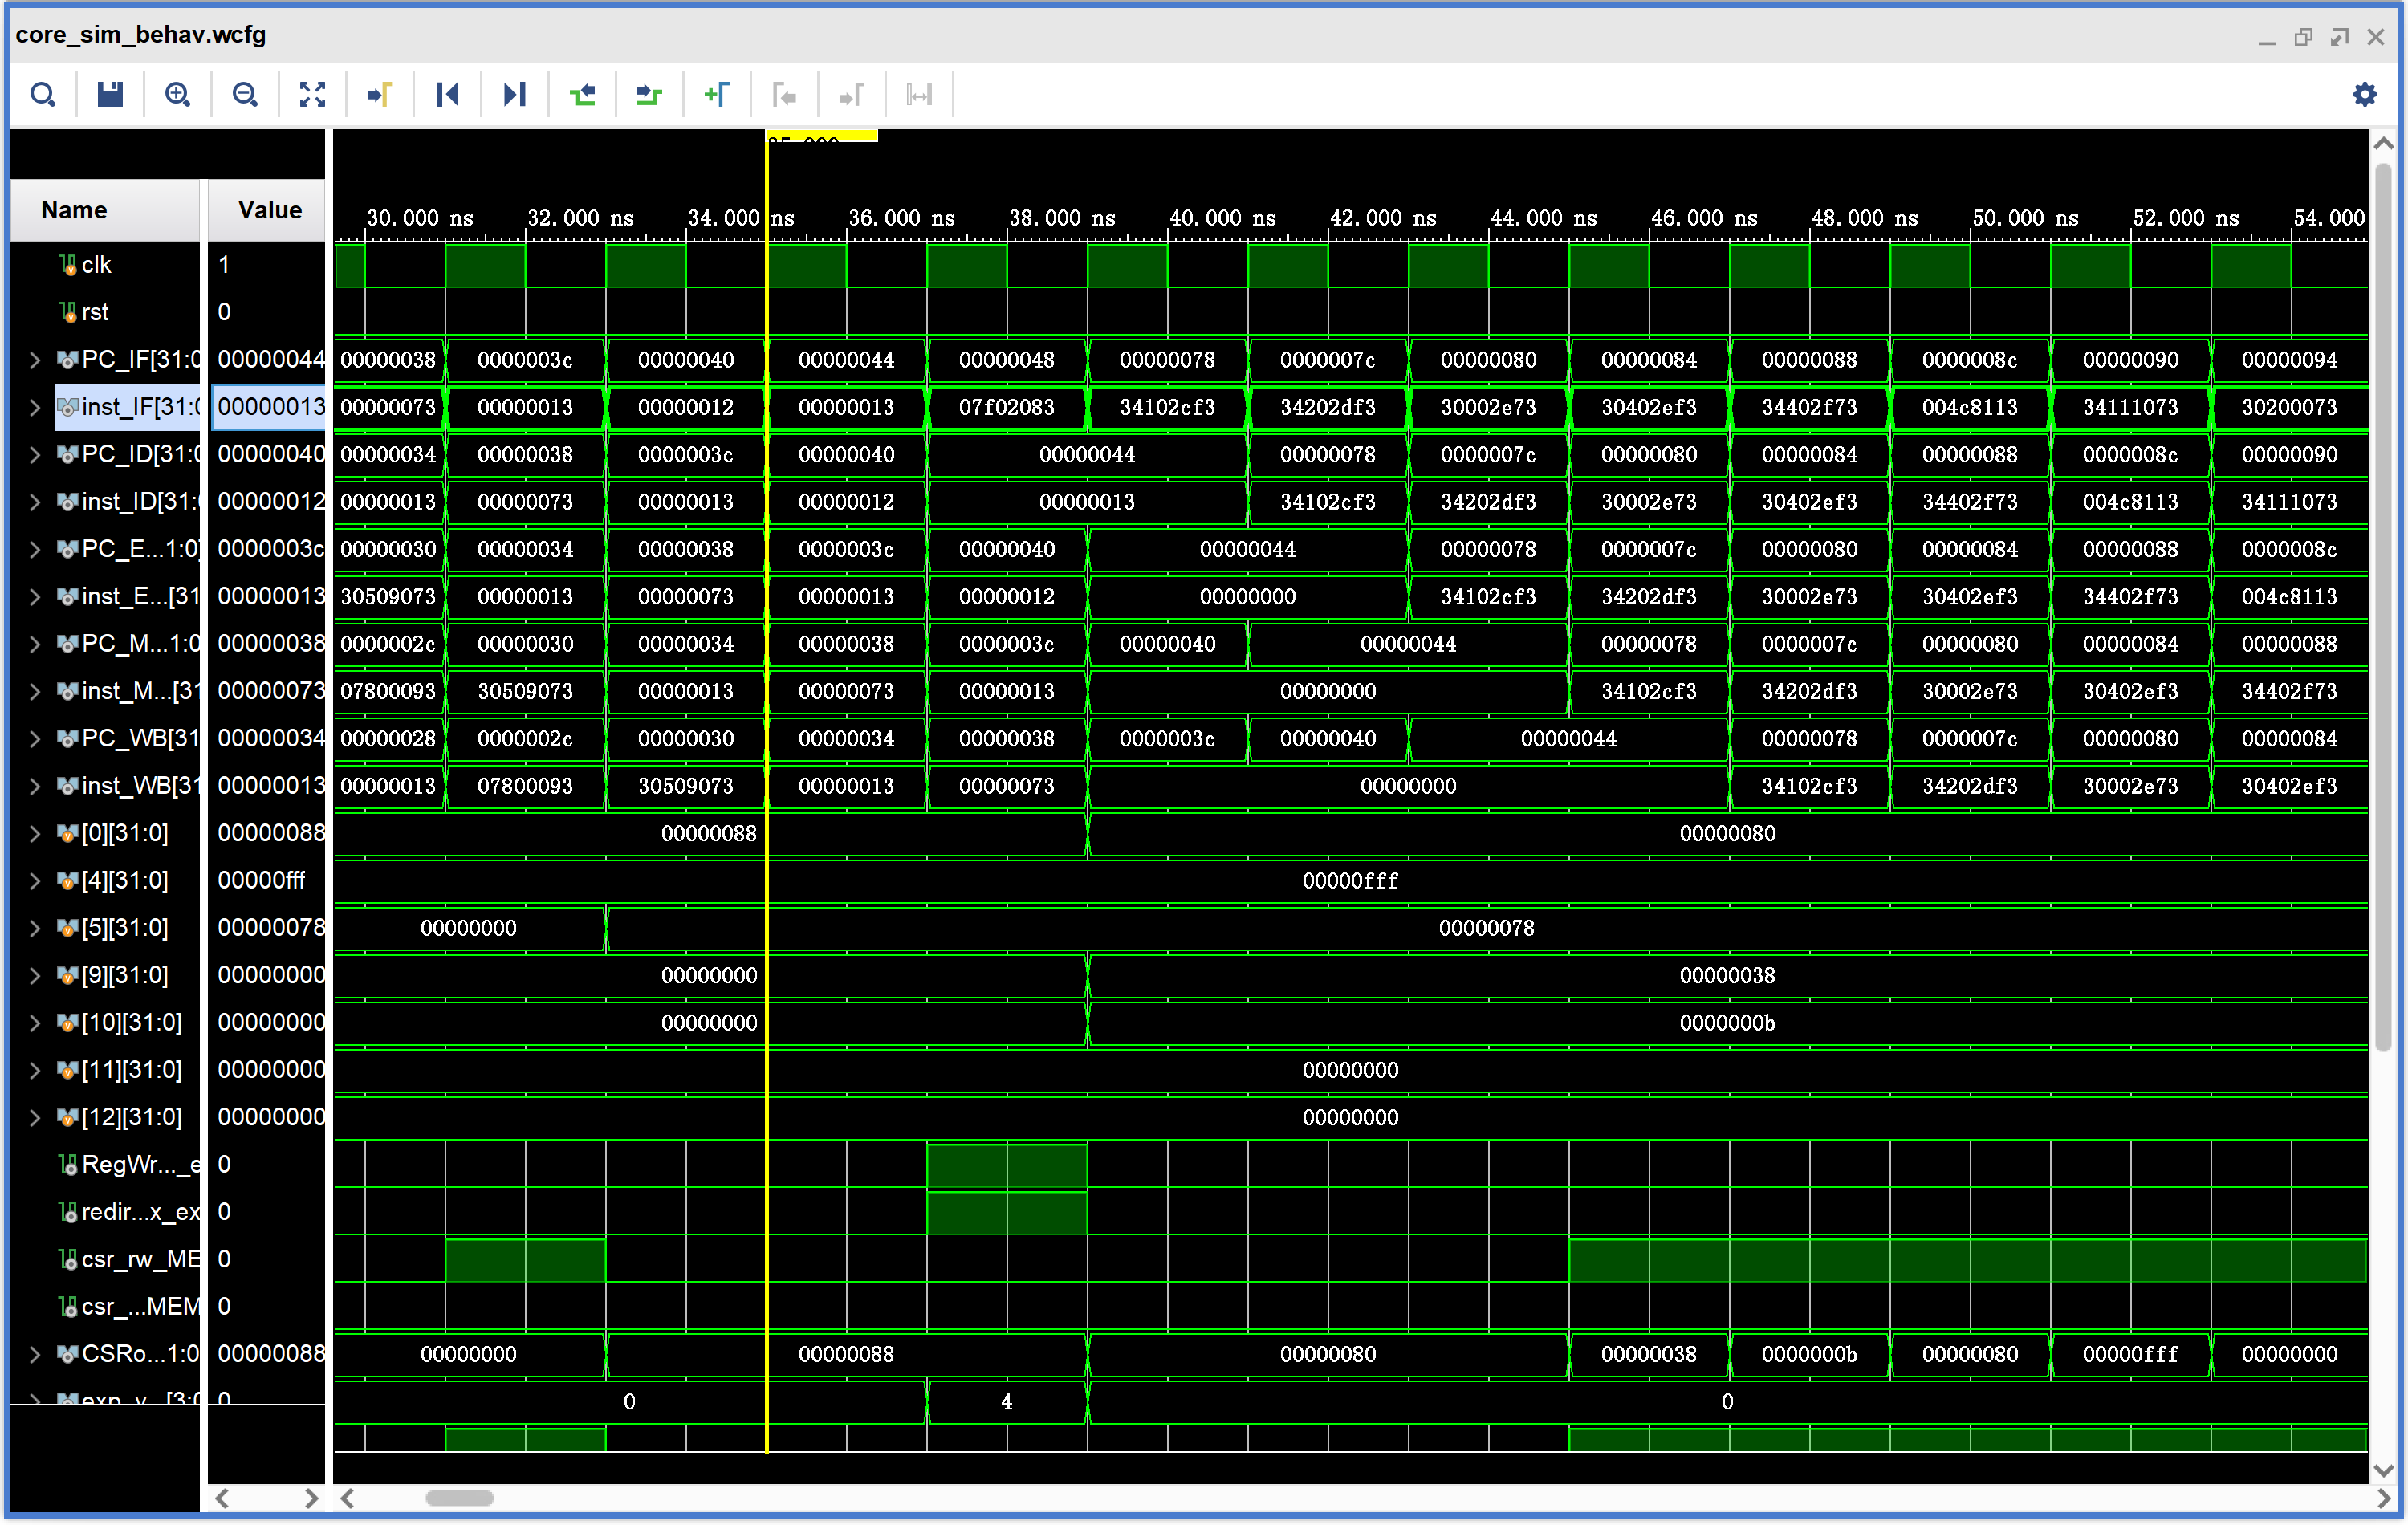
\includegraphics[width=1.0\textwidth]{figs/1.png} %插入图片,[]中设置图片大小,{}中是图片文件名
	\caption{仿真结果图1} %最终文档中希望显示的图片标题
	\label{Fig.11} %用于文内引用的标签
\end{figure}
当异常处理程序运行至末尾时,程序读取到mret指令并回到原程序中,由于在异常处理程序中给mepc加上了4,实际回到的是异常发生指令的下一条指令。
\begin{figure}[H] %H为当前位置,!htb为忽略美学标准,htbp为浮动图形
	\centering %图片居中
	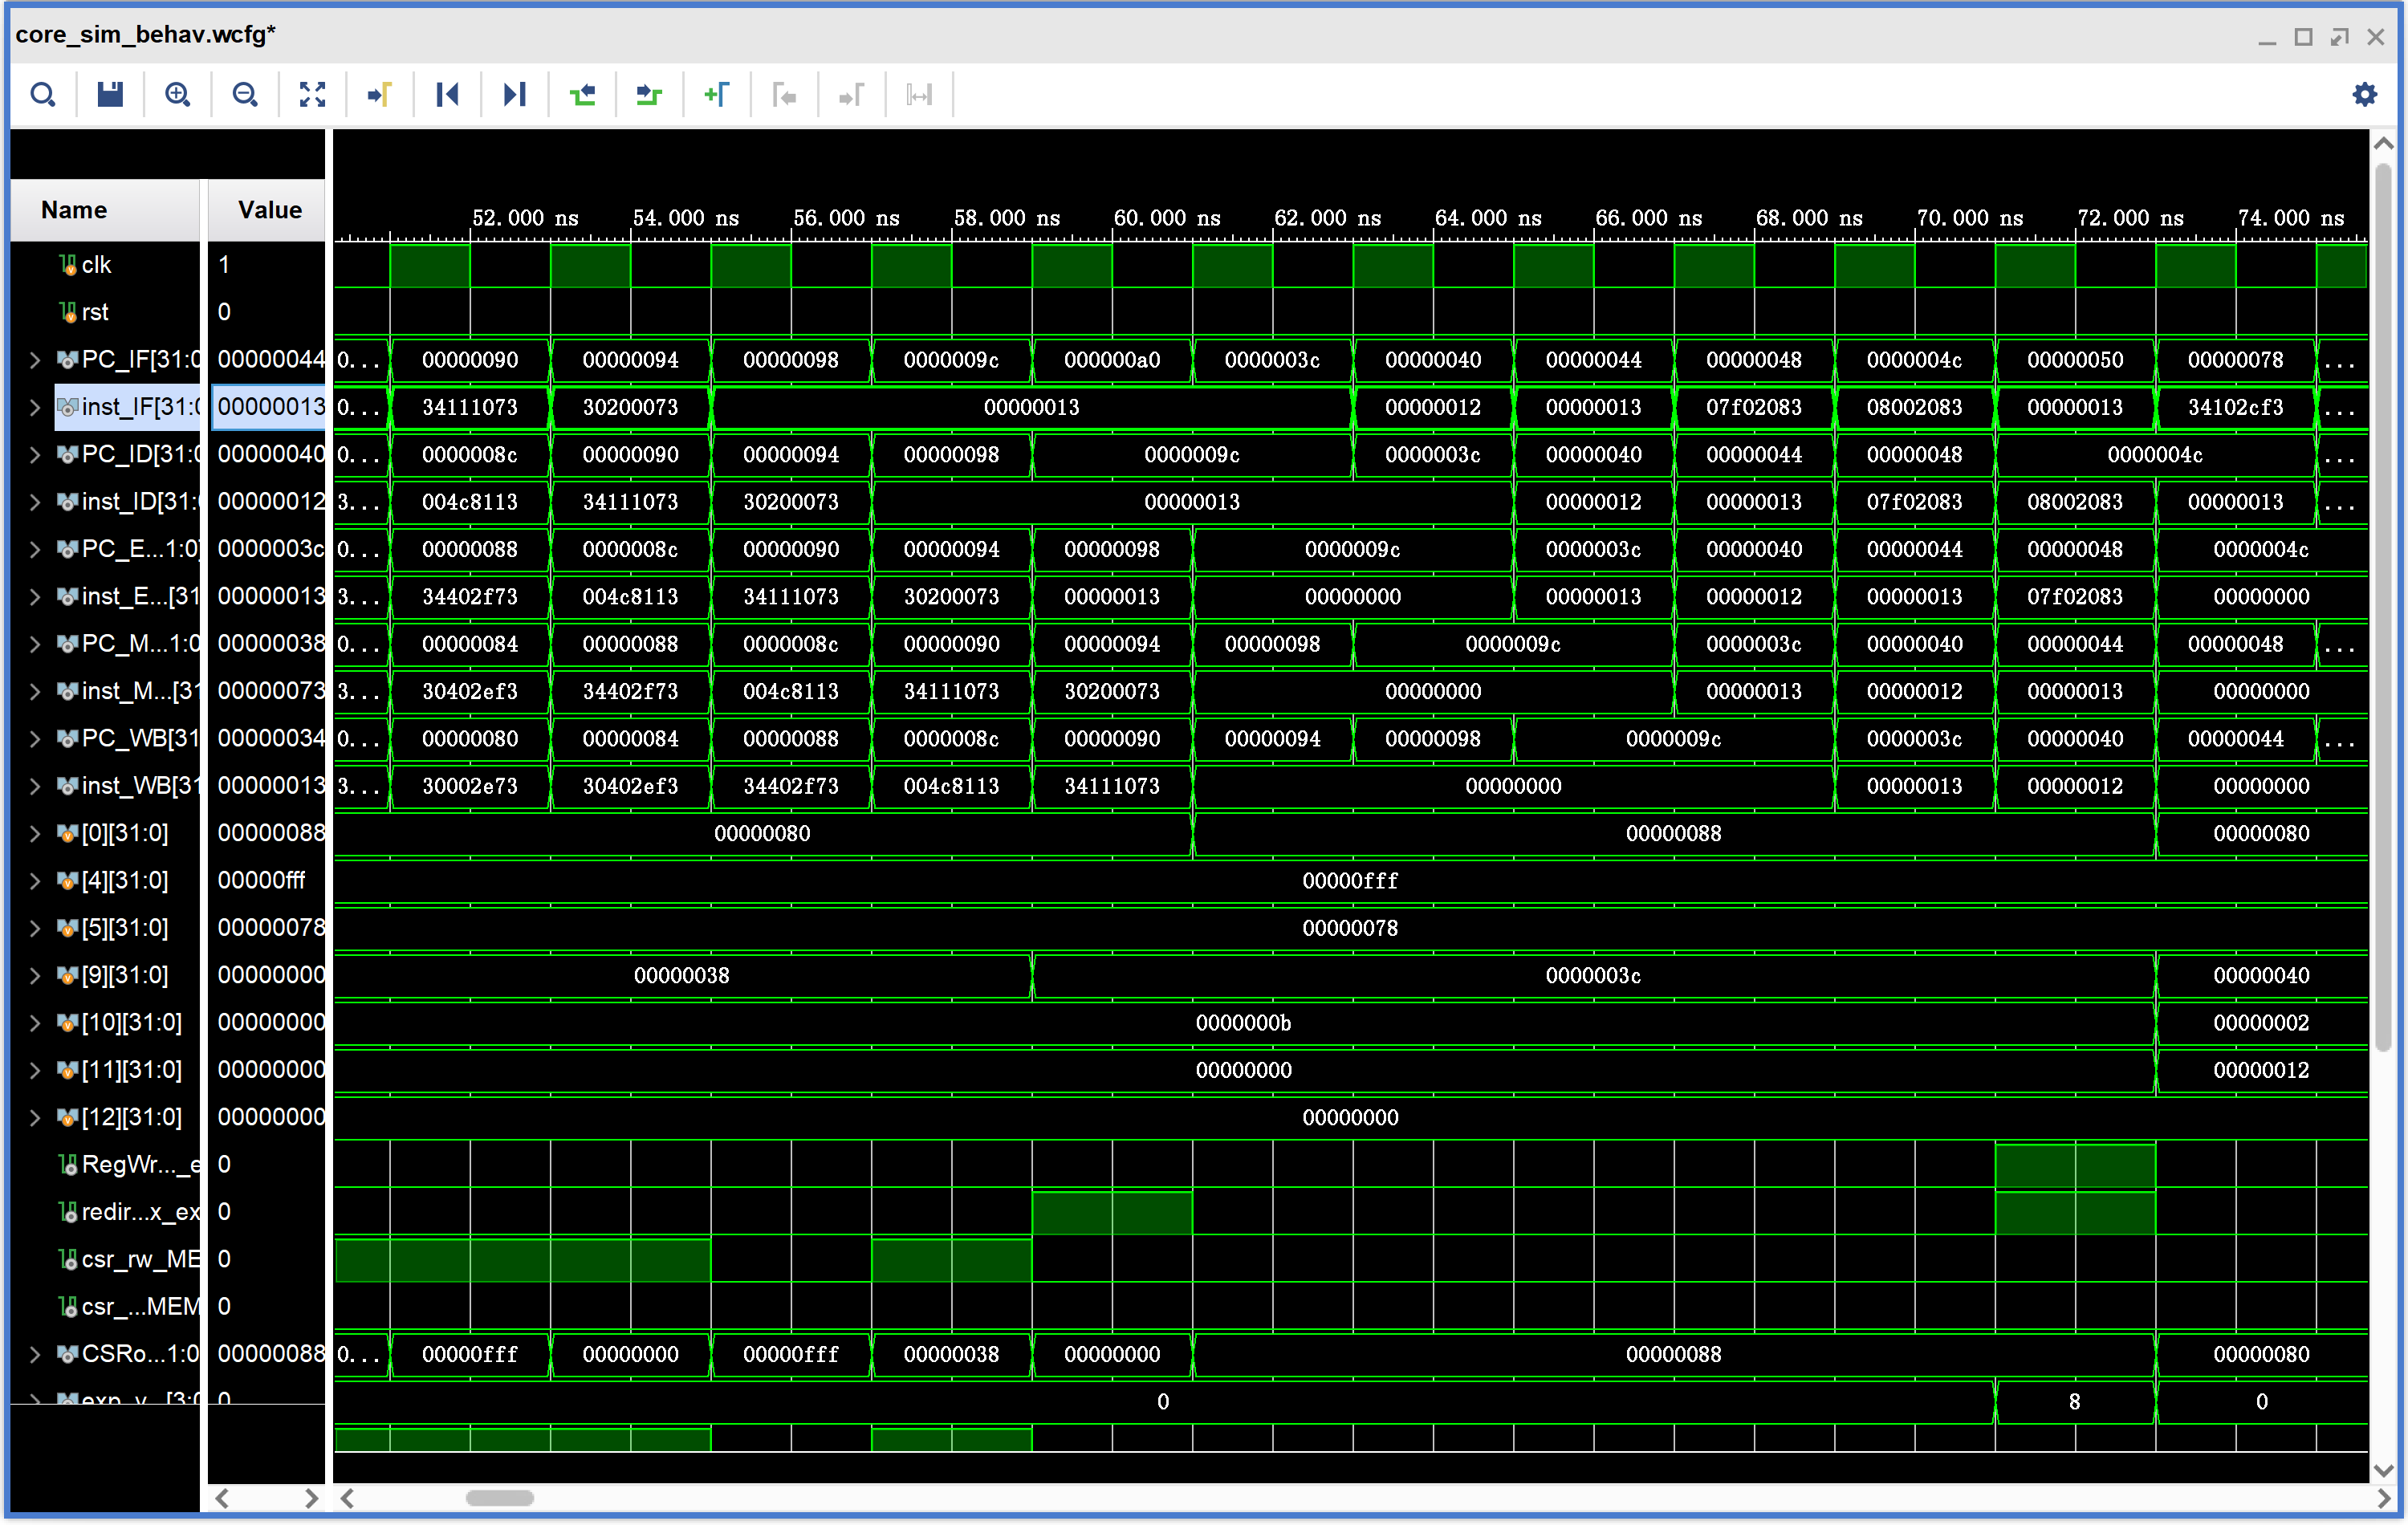
\includegraphics[width=1.0\textwidth]{figs/2.png} %插入图片,[]中设置图片大小,{}中是图片文件名
	\caption{仿真结果图2} %最终文档中希望显示的图片标题
	\label{Fig.12} %用于文内引用的标签
\end{figure}
之后程序继续运行直到遇到下一个异常,并以相同的方式处理该异常。
\begin{figure}[H] %H为当前位置,!htb为忽略美学标准,htbp为浮动图形
	\centering %图片居中
	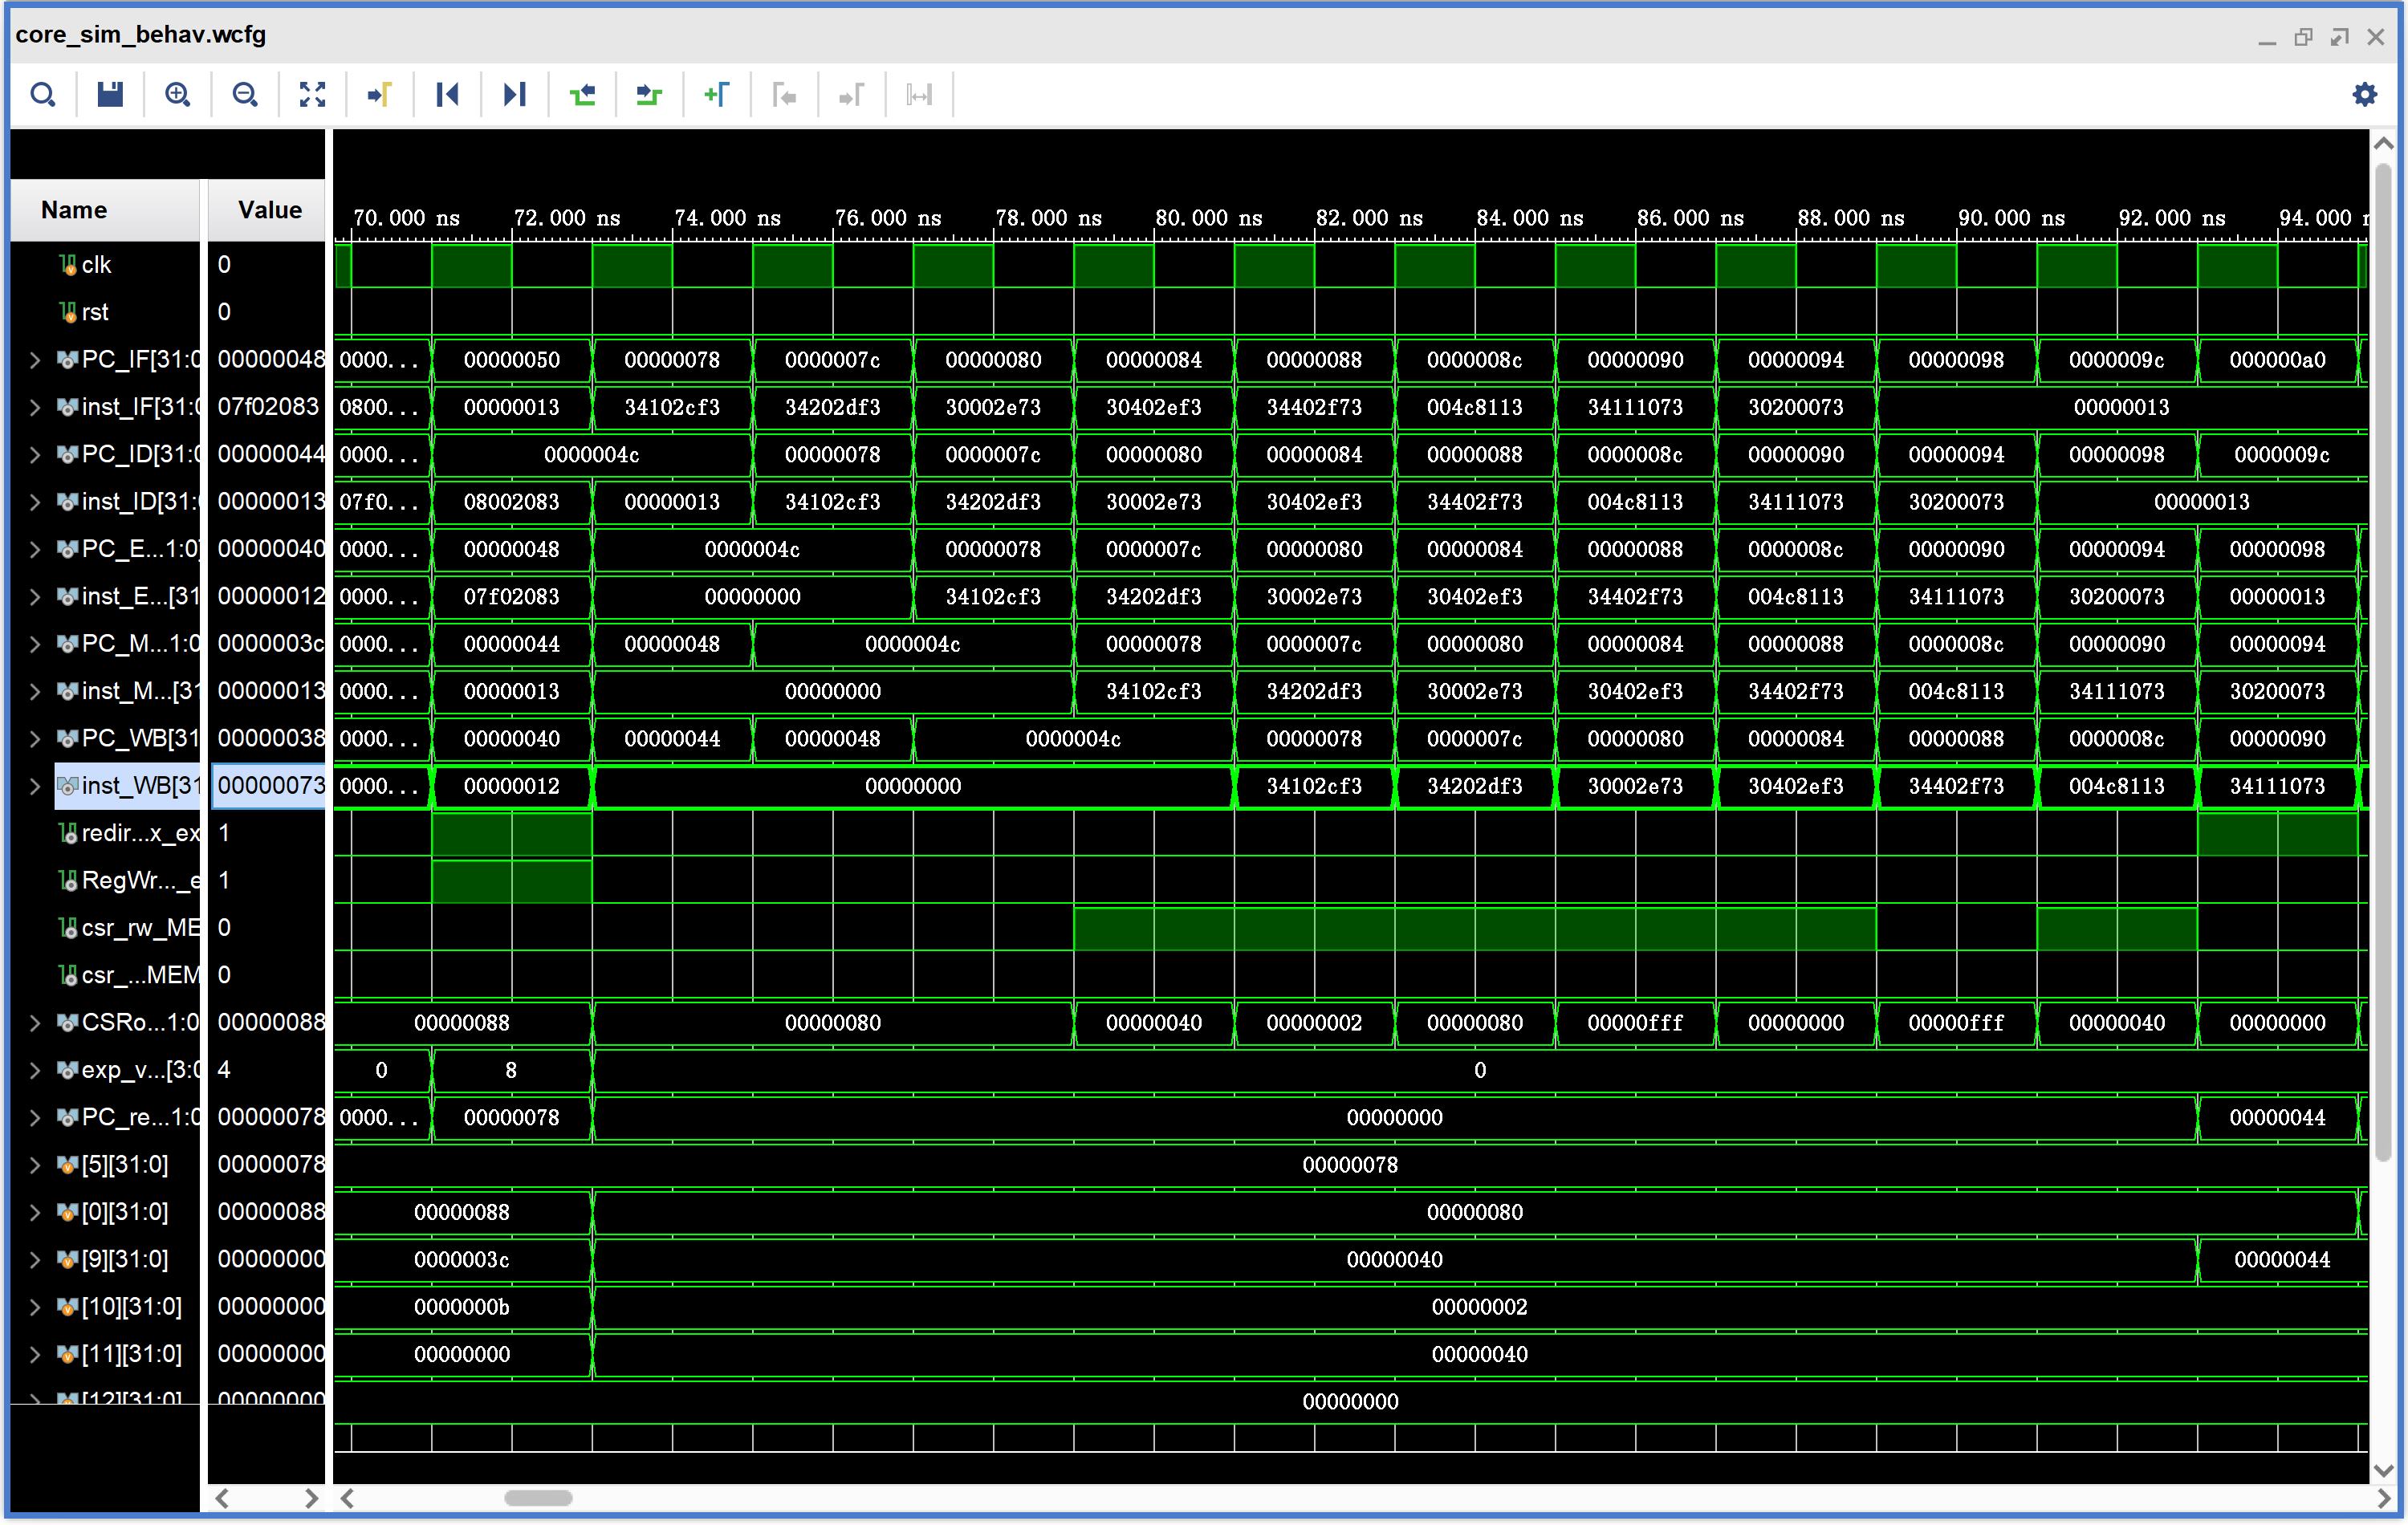
\includegraphics[width=1.0\textwidth]{figs/3.png} %插入图片,[]中设置图片大小,{}中是图片文件名
	\caption{仿真结果图3} %最终文档中希望显示的图片标题
	\label{Fig.13} %用于文内引用的标签
\end{figure}
\subsubsection{中断处理}
当程序遇到外部中断时,进入中断处理程序。在中断过程中,虽然中断信号一直拉起,但是由于mstatus的mie位此时为零,因此无法在中断中触发中断。
\begin{figure}[H] %H为当前位置,!htb为忽略美学标准,htbp为浮动图形
	\centering %图片居中
	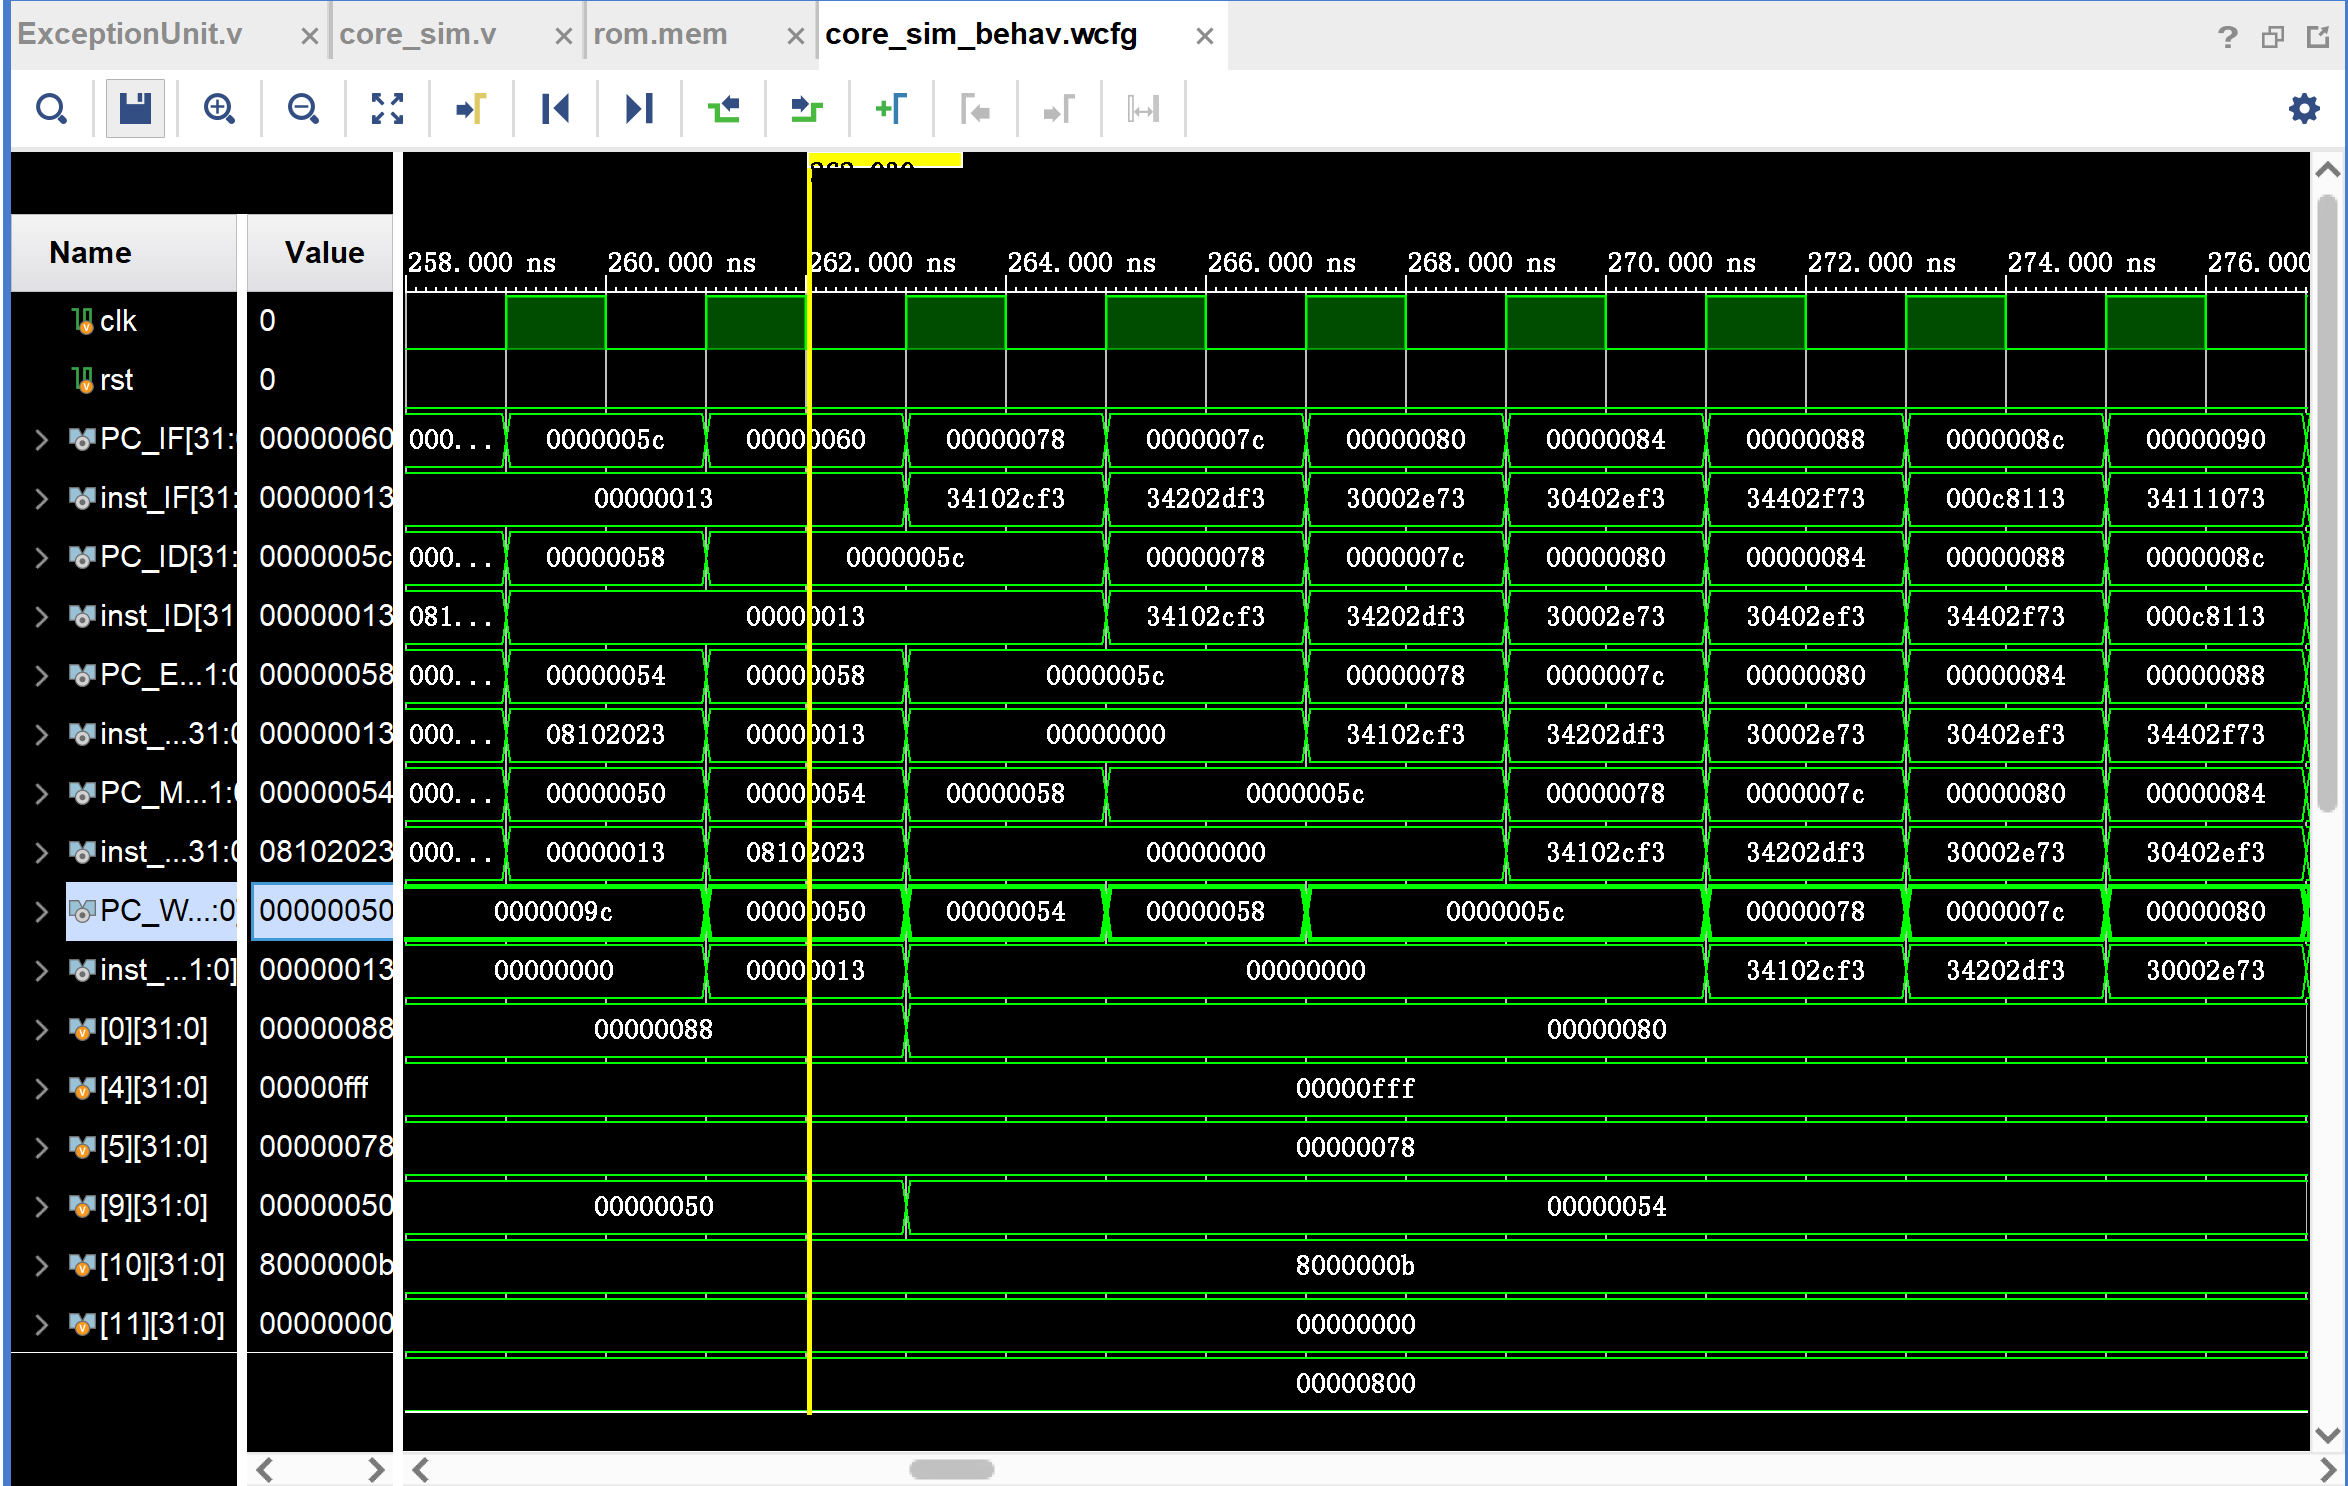
\includegraphics[width=1.0\textwidth]{figs/4.png} %插入图片,[]中设置图片大小,{}中是图片文件名
	\caption{仿真结果图4} %最终文档中希望显示的图片标题
	\label{Fig.14} %用于文内引用的标签
\end{figure}
返回时回到需要执行的下一条指令
\begin{figure}[H] %H为当前位置,!htb为忽略美学标准,htbp为浮动图形
	\centering %图片居中
	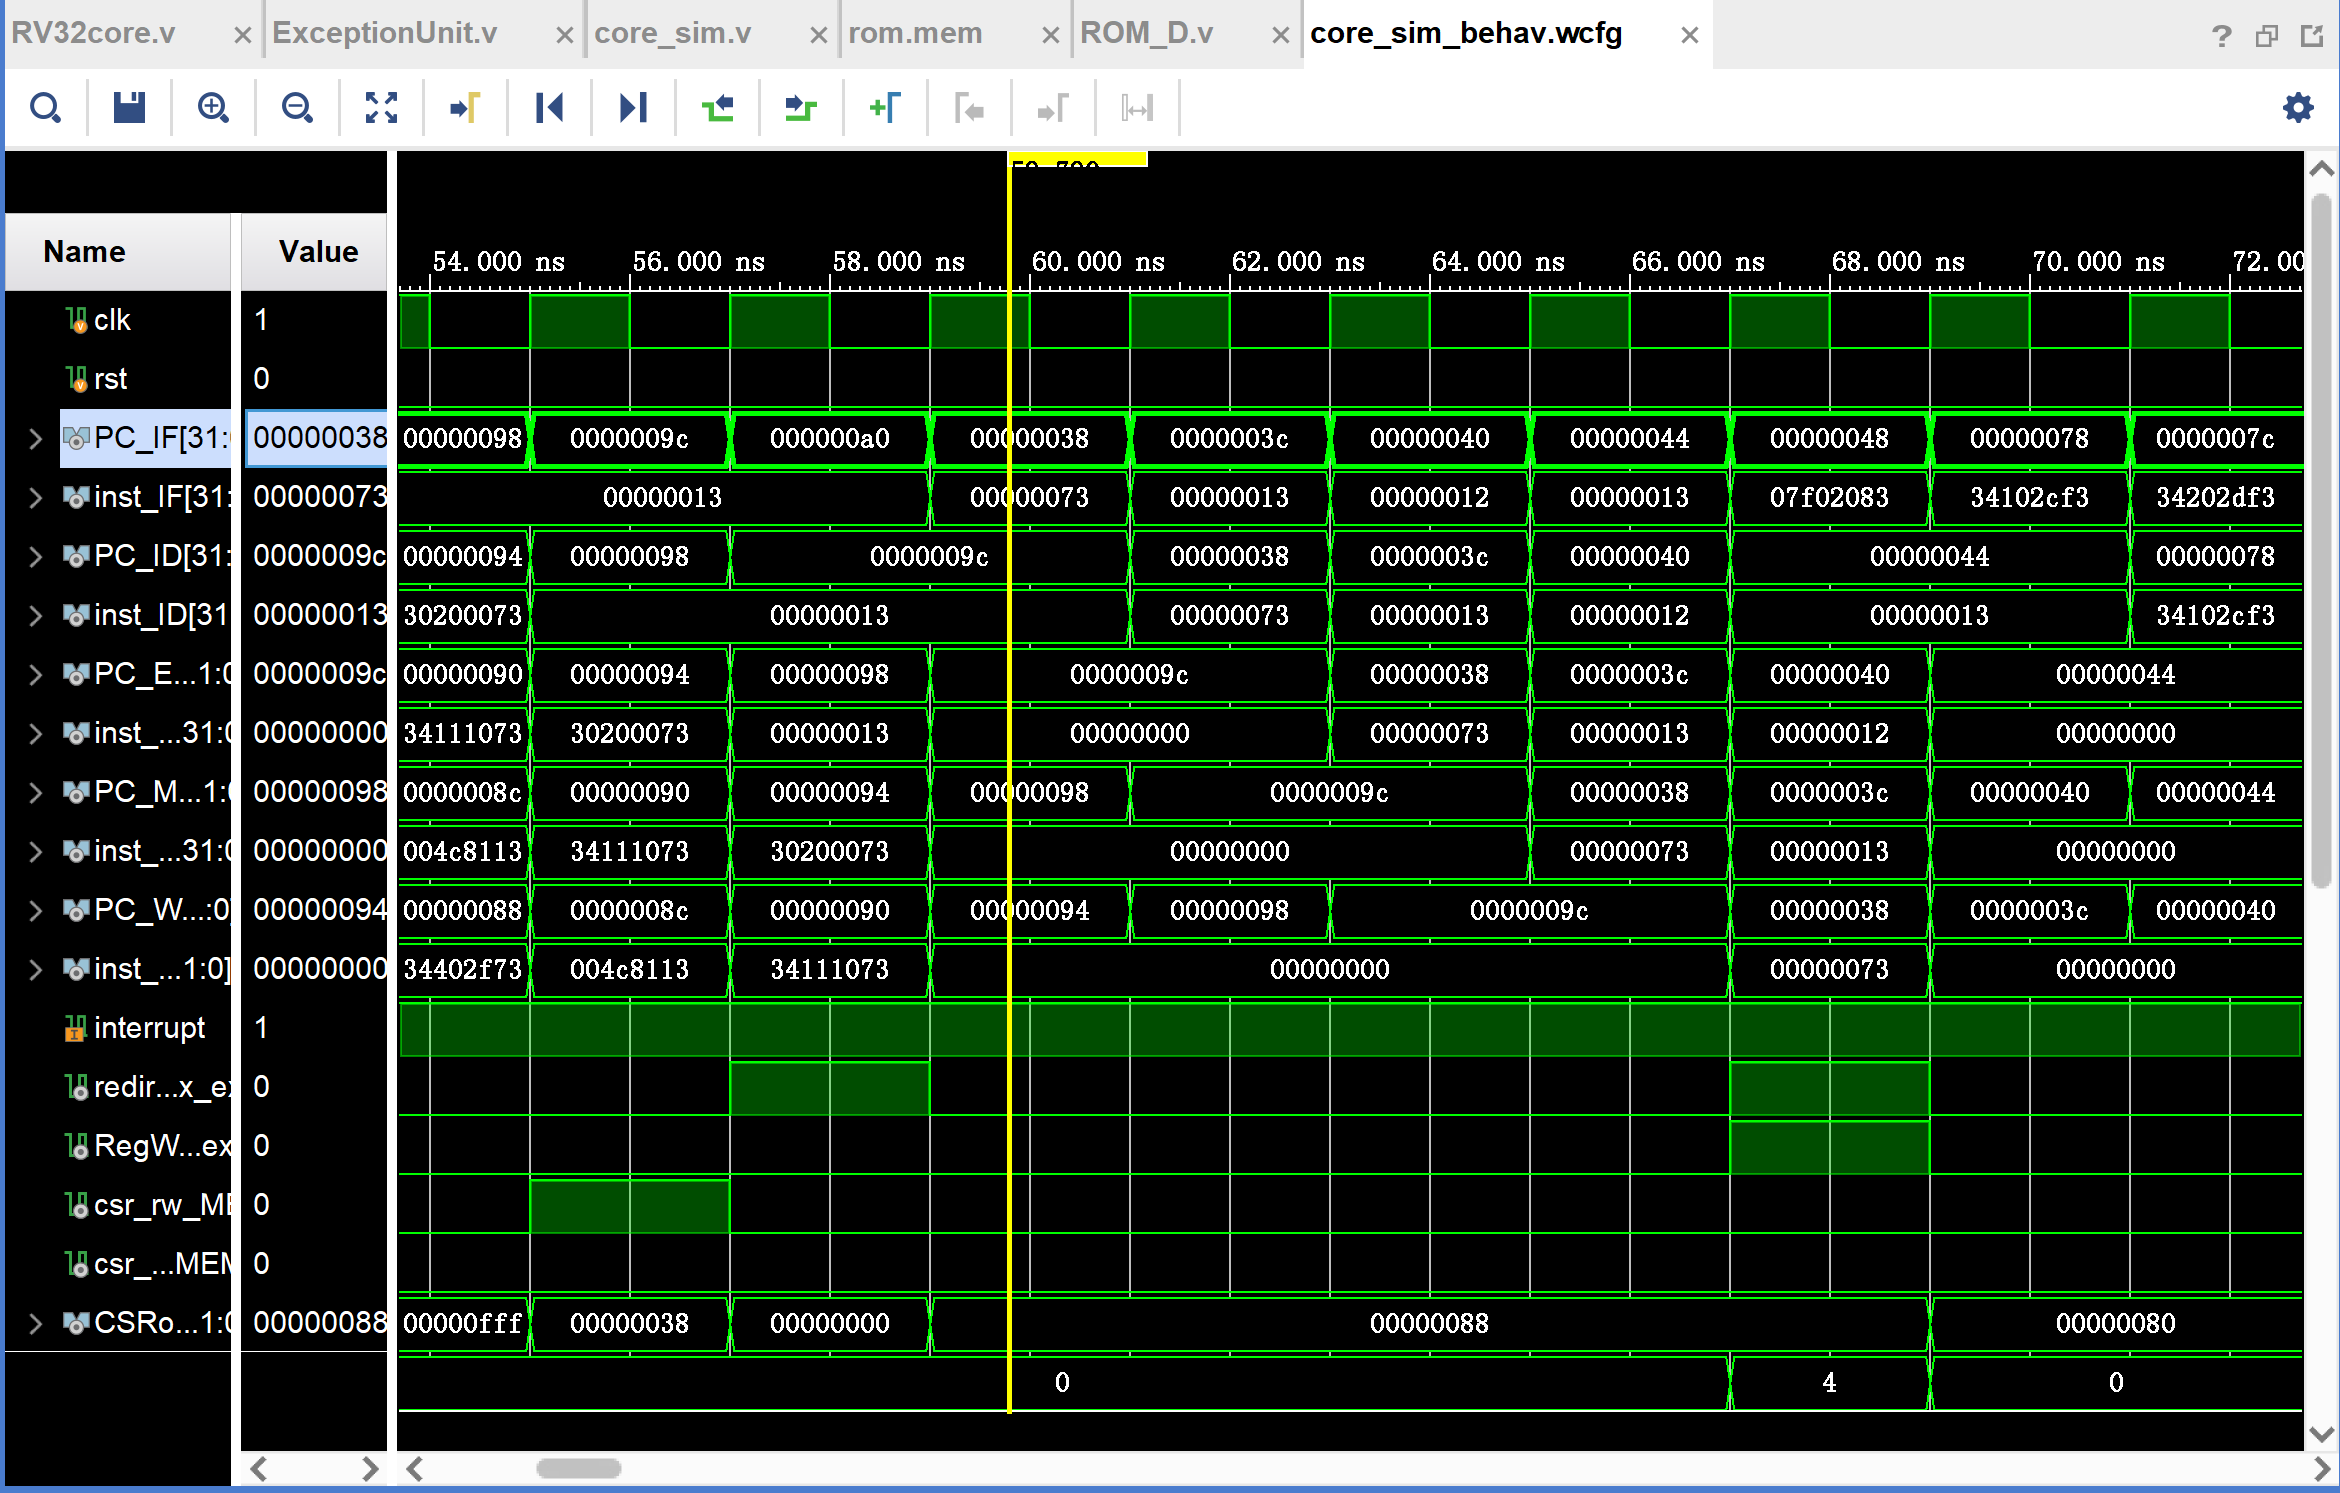
\includegraphics[width=1.0\textwidth]{figs/5.png} %插入图片,[]中设置图片大小,{}中是图片文件名
	\caption{仿真结果图5} %最终文档中希望显示的图片标题
	\label{Fig.15} %用于文内引用的标签
\end{figure}
返回后中断信号依旧处于拉起状态,在程序完全离开中断处理程序后,再次进入中断处理程序。
\begin{figure}[H] %H为当前位置,!htb为忽略美学标准,htbp为浮动图形
	\centering %图片居中
	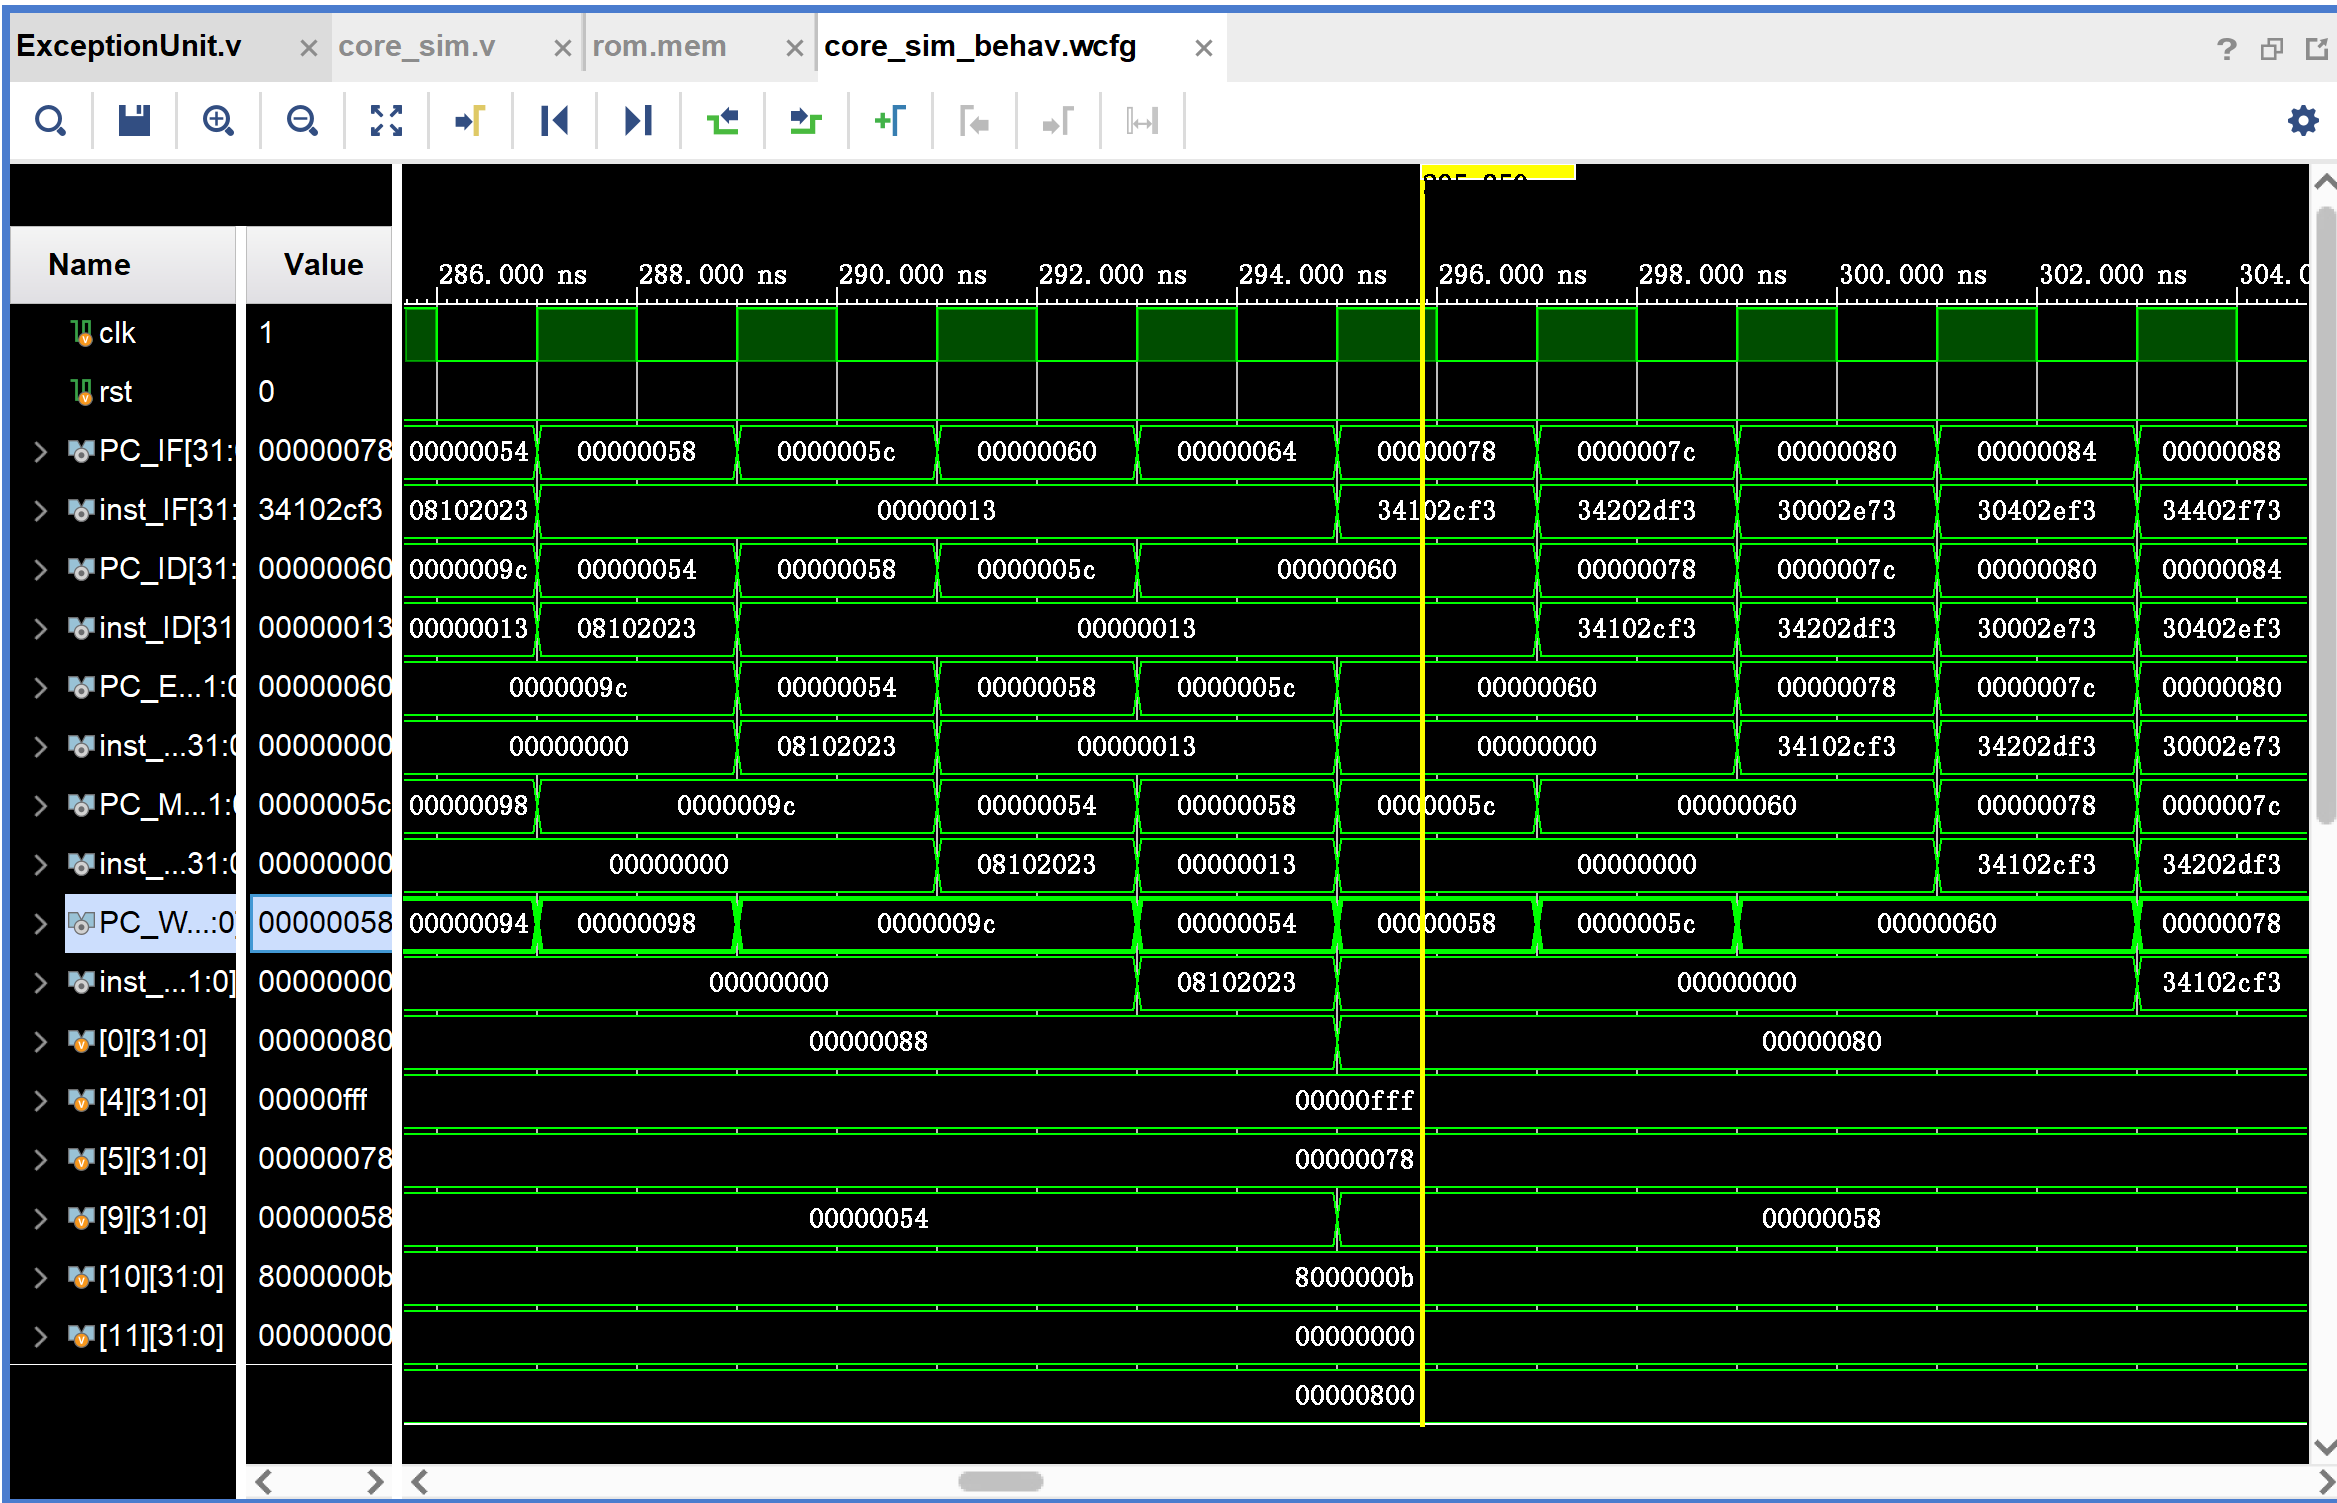
\includegraphics[width=1.0\textwidth]{figs/6.png} %插入图片,[]中设置图片大小,{}中是图片文件名
	\caption{仿真结果图6} %最终文档中希望显示的图片标题
	\label{Fig.16} %用于文内引用的标签
\end{figure}
\subsection{综合} 选择左侧面板的Run Synthesis或者点击上方的绿色小三角,选择Synthesis
\subsection{实现} 选择左侧面板的Run Implementation或者点击上方的绿色小三角,选择Implementation。值得注意的是执行implementation之前应该确保引脚约束存在且正确,同时之前已经综合过最新的代码。
\subsection{验证设计} 选择左侧面板的Open Elaborated Design,输出的结果如下,根据原理图来判断,基本没有问题
% \begin{figure}[H] %H为当前位置,!htb为忽略美学标准,htbp为浮动图形
%     \centering %图片居中
%     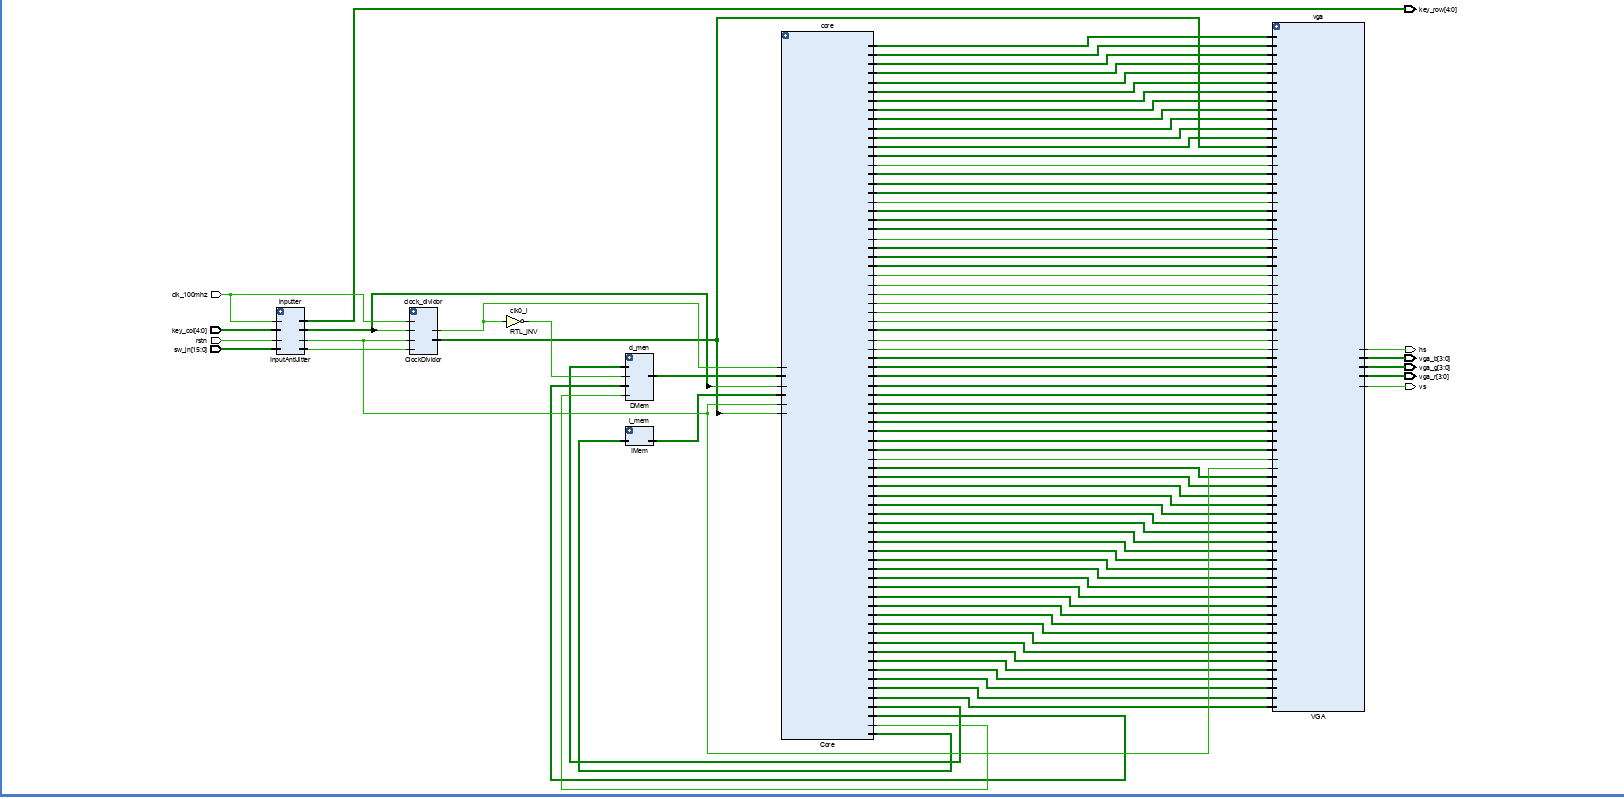
\includegraphics[width=1.0\textwidth]{yanzhen.png} %插入图片,[]中设置图片大小,{}中是图片文件名
%     \caption{验证结果图} %最终文档中希望显示的图片标题
%     \label{Fig.6} %用于文内引用的标签
% \end{figure}
\subsection{生成二进制文件} 选择左侧面板的Generate Bitstream或者点击上上的绿色二进制标志。同时生成Bitstream前要确保:之前已经综合、实现过最新的代码。如没有,直接运行会默认从综合、实现开始。此过程还要注意生成的bit文件默认存放在.runs下相应的implementation文件夹中
\subsection{烧写上板} 点击左侧的Open Hardware Manager $\rightarrow$ 点击Open Target $\rightarrow$ Auto Connect $\rightarrow$ 点击Program Device $\rightarrow$ 选择bistream路径,烧写。验证结果见实验结果部分。
